\section{Efficiency}\label{sec:efficiency}
Next to the correctness, the efficiency of the proposed method is the most important property to determine its feasibility. The main question is if or from what table size the proposed method is faster than the naive method. This becomes even more interesting as each positive guess of the model has to be verified using the naive algorithm to increase the accuracy.

The following experiments explore the efficiency of the proposed method in comparison to the naive algorithm and which parameters have the greatest influence on it.


\subsection{Experiment Data}\label{subsec:efficiency-experiment_data}
The experiments in this section were conducted on a set of generated tables to control the size of the table as well as the number of unique and non-unique columns. A small example of such a table can be seen in Table~\ref{table:efficiency-generated_table}.

Each generated table has \num{10} rows and between \num{100} and \num{100000000} columns. To ensure the correct prediction by the model, the columns where generated in a specific way.
The unique columns are evenly incrementing for the first \num{50} rows, while the first two rows of the non-unique columns contain the same value. The rest of each column contains distinct incrementing values which are mixed up to increase the time which the sorting based naive algorithm takes to find unique columns.

\begin{table}[!ht]
  {
    \newcommand{\tablevdots}{\multicolumn{1}{c}{\vdots{}}}
    \setlength{\tabcolsep}{5pt}
    \caption[A table generated for the efficiency experiment]{A table generated for the efficiency experiment. The columns 0 and 1 do not contain any duplicates, the columns 2, 3 and 4 do. To guarantee that the model guesses the unique and non-unique columns correctly, the unique columns are evenly incrementing for the first 50 rows, while the duplicate value of the non-unique columns is in the first two rows.}
    \begin{tabularx}{\linewidth}{X<{\centering}SSSSS}
      \toprule
      {Index}       & {Column \num{0}} & {Column \num{1}} & {Column \num{2}} & {Column \num{3}} & {Column \num{4}} \\ \midrule
      \num{0}       & 0                & 0                & 100              & 100              & 100              \\
      \num{1}       & 1                & 1                & 100              & 100              & 100              \\
      \num{2}       & 2                & 2                & 93               & 93               & 93               \\
      \num{3}       & 3                & 3                & 45               & 45               & 45               \\
      % 4        & 4                & 4                & 16               & 16               & 16               \\
      % 5        & 5                & 5                & 87               & 87               & 87               \\
      % 6        & 6                & 6                & 32               & 32               & 32               \\
      \tablevdots{} & \tablevdots{}    & \tablevdots{}    & \tablevdots{}    & \tablevdots{}    & \tablevdots{}    \\
      % 46       & 46               & 46               & 2                & 2                & 2                \\
      % 47       & 47               & 47               & 73               & 73               & 73               \\
      \num{48}      & 48               & 48               & 89               & 89               & 89               \\
      \num{49}      & 49               & 49               & 39               & 39               & 39               \\
      \num{50}      & 91               & 91               & 60               & 60               & 60               \\
      \num{51}      & 77               & 77               & 49               & 49               & 49               \\
      % 52       & 54               & 54               & 23               & 23               & 23               \\
      % 53       & 70               & 70               & 30               & 30               & 30               \\
      \bottomrule{}
    \end{tabularx}\label{table:efficiency-generated_table}

  }
\end{table}



\subsection{Base experiment}\label{subsec:efficiency-base_experiment}
The first experiment explores the efficiency of the proposed method compared to the naive algorithm. The generated tables that were used contained \num{3} unique and \num{7} non-unique columns.  % chktex 18

Figure~\ref{fig:efficiency-base_experiment-plot} and Table~\ref{table:efficiency_csv-70percent} show that for tables with up to \num{100000} rows, the naive algorithm takes only a fraction of a second and is therefore faster than the proposed machine learning model. However, since the model takes a roughly constant time of half a second to compute its prediction, it becomes faster as the table size surpasses one million rows.

The column \enquote{Model: Validation} in Table~\ref{table:efficiency_csv-70percent} additionally illustrates that the validation time of the proposed method is proportional to the number of positive guesses by the model. This highlights the importance of finding as few false positive guesses as possible because each false positive guess unnecessarily increases the runtime through the required validation and therefore decreases the efficiency.

In conclusion, this experiment illustrates that for large tables loading the dataset and checking the columns for duplicates with the naive algorithm takes the most time. Possibilities to reduce the loading time will be explored in Section~\ref{subsec:efficiency-shorter_loading_times}. While a more efficient naive algorithm is not part of this thesis, Section~\ref{subsec:correctness_comparing-input-size} and~\ref{subsec:correctness_examine-false-guesses} deal with the question of how to decrease the number of false positive guesses.

\begin{figure}[ht]
  \caption[Compare the efficiency the proposed method and the naive algorithm]{This plot shows the total time for the naive algorithm and the proposed method to compute the unique columns as can be seen in Table~\ref{table:efficiency_csv-70percent}. The tables were saved in a CSV format.} % TODO: better caption
  \label{fig:efficiency-base_experiment-plot} % chktex 24
  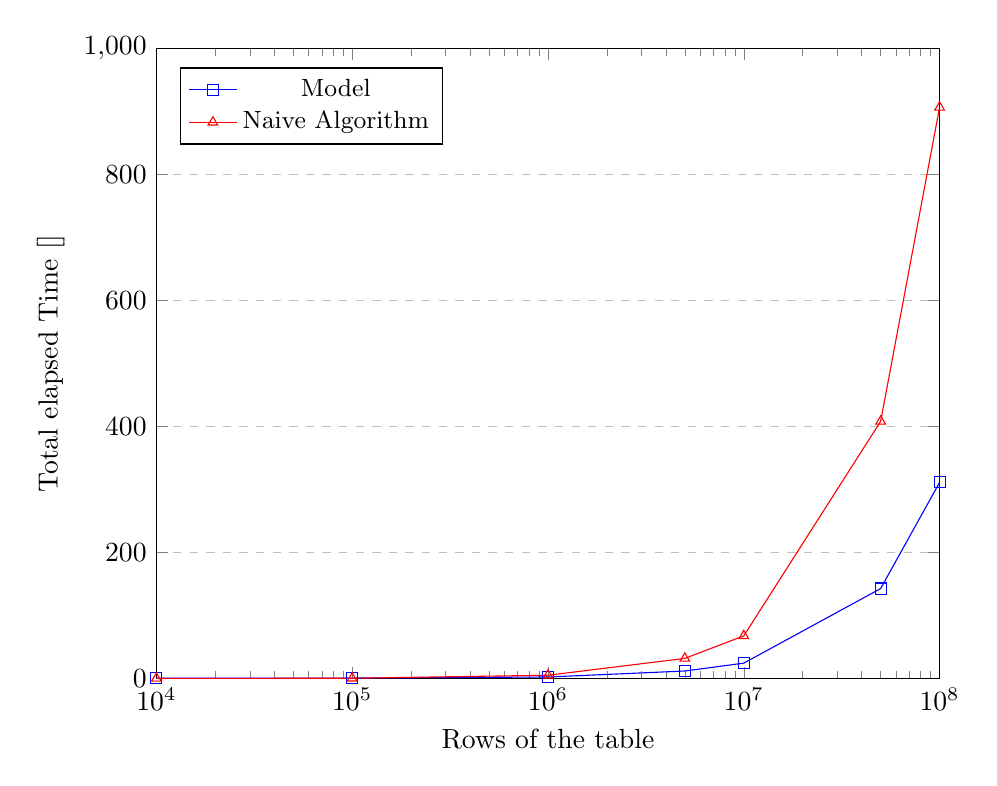
\begin{tikzpicture}
    \begin{axis}[
        % title={},
        xlabel={Rows of the table},
        ylabel={Total elapsed Time [\si{\second}]},
        xmin=10000, xmax=100000000, xmode=log,
        ymin=0, ymax=1000,
        % xtick={0,1000,100000,10000000,100000000},
        % ytick={0,20,40,60,80,100,120},
        legend pos=north west,
        ymajorgrids=true,
        grid style=dashed,
        scale only axis,
        width={\linewidth-62pt},
        height=8cm
      ]

      \addplot[
        color=blue,
        mark=square,
      ]
      coordinates {
          (100.0,1.0835406184196472) (1000.0,0.4514627978205681) (10000.0,0.4591604061424732) (100000.0,0.5741918832063675) (1000000.0,2.2600879333913326) (5000000.0,11.771335251629353) (10000000.0,24.25790297240019) (50000000.0,142.64984269440174) (100000000.0,311.1732710637152)
        };
      \addplot[
        color=red,
        mark=triangle,
      ]
      coordinates{
          (100.0,0.0039823874831199) (1000.0,0.0037141181528568) (10000.0,0.0264939442276954) (100000.0,0.3022922314703464) (1000000.0,5.0495885498821735) (5000000.0,31.796920645982027) (10000000.0,67.54112743958831) (50000000.0,408.1332451477647) (100000000.0,906.6464131213723)
        };
      \legend{\small Model, \small Naive Algorithm}

    \end{axis}
  \end{tikzpicture}
\end{figure}


\begin{table}[htb]
    \centering
    \begin{tabular}{@{}cccccccccc@{}}
        \toprule
        Rows & Columns & ML: Loading & ML: Compute Time & ML: Loading & ML: Validation Time & ML: Total & Naive: Loading & Naive: Compute Time & Naive: Total \\
        \midrule
        100 & 10 & 0.0065117068588733 & 1.901446133852005 & 0.0065117068588733 & 0.0001417063176631 & 1.90841730684042 & 0.0035603828728199 & 0.0005022697150707 & 0.0040644854307174 \\
        1000 & 10 & 0.0015828944742679 & 1.8984689489007 & 0.0015828944742679 & 0.0006108358502388 & 1.9009892046451569 & 0.0016751401126384 & 0.0019342266023159 & 0.0036102943122386 \\
        10000 & 10 & 0.0052565038204193 & 1.9095683731138704 & 0.0052565038204193 & 0.0065431855618953 & 1.921698283404112 & 0.0049404129385948 & 0.0220178365707397 & 0.0269592814147472 \\
        100000 & 10 & 0.0429374687373638 & 1.9027229472994804 & 0.0429374687373638 & 0.0742254443466663 & 2.020440120249986 & 0.0424283891916275 & 0.2558906264603138 & 0.2983216643333435 \\
        1000000 & 10 & 0.4255336932837963 & 1.903101004660129 & 0.4255336932837963 & 1.3649001717567444 & 3.696124318987131 & 0.4222380295395851 & 4.689979210495949 & 5.112221155315638 \\
        10000000 & 10 & 4.559976447373629 & 1.8975738510489464 & 4.559976447373629 & 19.02081367000937 & 25.518052734434605 & 4.547631841152906 & 63.52510995417833 & 68.0727454200387 \\
        100000000 & 10 & 51.986212998628616 & 1.90036316588521 & 51.986212998628616 & 257.835216768086 & 312.1136333048344 & 52.16438018530607 & 852.7149710021913 & 904.8793550543488 \\
        5000000 & 10 & 2.4457033053040504 & 1.8983104377985 & 2.4457033053040504 & 8.743456106632948 & 13.107568178325891 & 2.4423254802823067 & 29.05716192722321 & 31.49949196726084 \\
        50000000 & 10 & 26.75338465720415 & 1.89099595323205 & 26.75338465720415 & 114.87536582350732 & 143.71518944576383 & 27.03932445123792 & 379.5964986868202 & 406.6358272023499 \\
        \bottomrule
    \end{tabular}
\end{table}


\subsection{Reducing loading times}\label{subsec:efficiency-shorter_loading_times}
While CSV files are very easy to use, they are not meant to efficiently store large quantities of data. A file format which is substantially more suitable to handle large datasets is the parquet format~\cite{parquet-book}.

It achieves this through the use of various features such as column wise compression, which tends to be more efficient since the values in the same column are usually very similar. This has the additional benefit of enabling the algorithm to only read the required columns which may decrease \io{} as only positive guesses need to be loaded for the validation.

Another advantageous property of this format is the concept of row groups, which ensure that a batch of rows is being saved together and can therefore be read together too. This makes it possible to read just the first row group and use these rows as an input for the model.

Table~\ref{table:efficiency_parquet-70percent} shows the result of the base experiment from Section~\ref{subsec:efficiency-base_experiment} repeated with tables generated as parquet files. While the computing time for the model and the naive algorithm remain roughly equal compared to Table~\ref{table:efficiency_csv-70percent}, the loading time is decreased significantly for large tables. %? loading times make up a larger part of total time for model

Table~\ref{table:efficiency_parquet-70percent_small-tables} presents the result for the experiment using the advantages of the file format by loading only the necessary rows and columns. This leads to two loading times for the model. The first time only the first row group is being loaded while the second time only the columns which are unique according to the model are loaded. However, this does not make any difference except for the largest table and even then the total time is hardly changing.

\GenericWarning{}{LaTeX Warning: This table needs to be manually checked}
\begin{table}[ht]
    \caption{The result of the efficiency test with a generated table with \SI{30}{\percent} unique columns in a parquet file format. The test was conducted on a model with an input size of 10 rows on tables with 10 columns.}
    \begin{tabular}{@{}SSSSSSSSS@{}}
        \toprule
        {\shortstack{Rows}} & {\shortstack{Model:\\Loading}} & {\shortstack{Model:\\Computing}} & {\shortstack{Model:\\Loading}} & {\shortstack{Model:\\Validation}} & {\shortstack{Model:\\Total}} & {\shortstack{Naive:\\Loading}} & {\shortstack{Naive:\\Computing}} & {\shortstack{Naive:\\Total}} \\
        \midrule
        100 & 0.0037329792976379 & 0.4535947442054748 & 0.0037329792976379 & 0.0001380555331707 & 0.4577647559344768 & 0.0056636519730091 & 0.0005674697458744 & 0.0062335357069969 \\
        1000 & 0.002842117100954 & 0.4445352330803871 & 0.002842117100954 & 0.0006063096225261 & 0.4482727721333504 & 0.0034207440912723 & 0.0018974170088768 & 0.0053194314241409 \\
        10000 & 0.003845926374197 & 0.4464297965168953 & 0.003845926374197 & 0.0065436139702796 & 0.4571339413523674 & 0.0040172487497329 & 0.0205030031502246 & 0.0245211236178874 \\
        100000 & 0.0095696412026882 & 0.4469785206019878 & 0.0095696412026882 & 0.0770864151418209 & 0.5343325138092041 & 0.0097010508179664 & 0.2462445013225078 & 0.2559473849833011 \\
        1000000 & 0.0399911925196647 & 0.462495107203722 & 0.0399911925196647 & 1.3958711363375187 & 1.90179156512022 & 0.0468120314180851 & 4.618332322686911 & 4.6651470102369785 \\
        5000000 & 0.1967337541282177 & 1.2639095708727837 & 0.1967337541282177 & 8.750608161091805 & 10.232811015099289 & 0.183550912886858 & 29.032910093665123 & 29.216464921832085 \\
        10000000 & 0.4818546883761883 & 0.4799107164144516 & 0.4818546883761883 & 18.93440898507833 & 19.938058882951736 & 0.5291252098977566 & 62.745562482625246 & 63.27469082176685 \\
        50000000 & 2.216078583151102 & 0.9870042651891708 & 2.216078583151102 & 113.88575321435928 & 117.29449190944432 & 2.2049838453531265 & 379.4684140905738 & 381.673400811851 \\
        100000000 & 4.47317860648036 & 1.5488394163548946 & 4.47317860648036 & 257.4711396209896 & 263.89783180877566 & 4.395280238240957 & 857.4373284652829 & 861.8326124921441 \\
        \bottomrule
    \end{tabular}\label{table:efficiency_parquet-70percent}
\end{table}

\begin{table}[ht]
    \caption[Efficiency experiment on tables with \SI{30}{\percent} unique columns saved as parquet files, where only the necessary rows and columns are loaded]{The result of the efficiency experiment conducted on a table generated with \num{3} unique and \num{7} non-unique columns saved as a parquet file. The experiment was conducted on a model with an input size of 10 rows which was trained on the training dataset. During the experiment, only the necessary rows and columns were loaded.}
    \small
    \setlength{\tabcolsep}{4pt}
    \makebox[\linewidth][r]{%
        \begin{tabular}{@{}S[table-format=9]SSSSSSSS@{}}
            \toprule
            {\shortstack{Rows}} & {\shortstack{Model:\\Loading I}} & {\shortstack{Model:\\Computing}} & {\shortstack{Model:\\Loading II}} & {\shortstack{Model:\\Validation}} & {\shortstack{Model:\\Total}} & {\shortstack{Naive:\\Loading}} & {\shortstack{Naive:\\Computing}} & {\shortstack{Naive:\\Total}} \\
            \midrule
            100                 & 0.0019583702087402  & 0.4582597687840462 & 0.0025078989565372 & 0.0001805499196052 & 0.4629099182784557 & 0.0035582929849624 & 0.0004192851483821 & 0.0039786621928215 \\
            1000                & 0.0015548579394817  & 0.4559830017387867 & 0.0025322996079921 & 0.0007521696388721 & 0.4608258455991745 & 0.0026408433914184 & 0.0018298886716365 & 0.0044715628027915 \\
            10000               & 0.0024227760732173  & 0.4511252082884311 & 0.0029931813478469 & 0.0066407360136508 & 0.4631855227053165 & 0.0039258524775505 & 0.0203023217618465 & 0.024229060858488  \\
            100000              & 0.0093600116670131  & 1.4681769870221617 & 0.006388496607542  & 0.0805302299559116 & 1.5644594952464104 & 0.0085682570934295 & 0.2470835894346237 & 0.2556539326906204 \\
            1000000             & 0.0322037003934383  & 0.454765647649765  & 0.0255185328423976 & 1.356141496449709  & 1.8686350099742413 & 0.0499729178845882 & 4.665698669850826  & 4.715674605220556  \\
            5000000             & 0.1148154400289058  & 0.4625117443501949 & 0.1057574264705181 & 8.687994543462992  & 9.371084868907928  & 0.1949679963290691 & 29.00083852931857  & 29.195809934288263 \\
            10000000            & 0.2425682730972767  & 0.4470147676765919 & 0.2583311088383198 & 18.96086385846138  & 19.90878576785326  & 0.5438475236296654 & 63.12243377417326  & 63.66628506034613  \\
            50000000            & 1.1834049336612225  & 0.447280365973711  & 1.3086804077029228 & 114.8945118971169  & 117.83388417959212 & 2.2251016534864902 & 379.7313333004713  & 381.9564390294254  \\
            100000000           & 1.6024668291211128  & 0.4462943933904171 & 2.42531206831336   & 256.9933520145714  & 261.4674338325858  & 4.437270112335682  & 856.736768040806   & 861.1740412451327  \\
            \bottomrule
        \end{tabular}\label{table:efficiency_parquet-70percent_small-tables}
    }
\end{table}

In summary, while the reduced loading time does make a notable difference, it is not very large compared to the efficiency gain achieved through the use of the proposed method, which is additionally demonstrated in Figure~\ref{fig:efficiency-shorter_loading_time-plot}. This could change, however, if the file reading speed would be slower, for example because the data had to be read over the internet. In this case, reading only the necessary rows and columns and thus decreasing \io{} further could make a larger difference too.

\begin{figure}[ht]
  \caption[]{} %! TODO: better caption
  \label{fig:efficiency-shorter_loading_time-plot} % chktex 24
  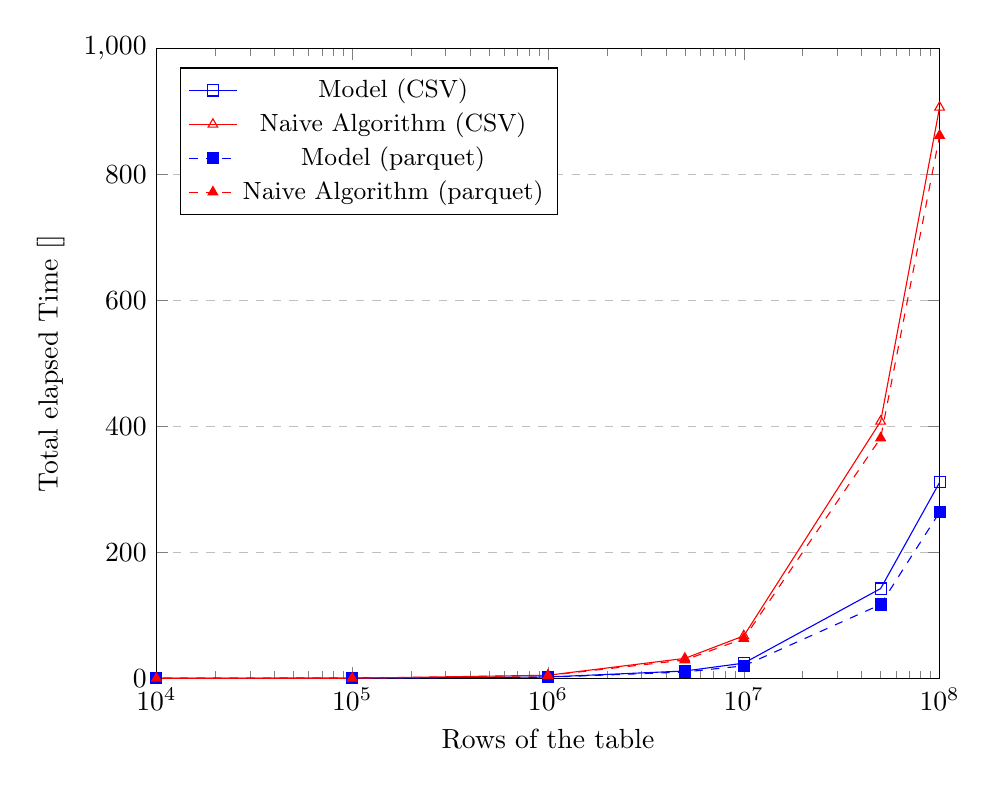
\begin{tikzpicture}
    \begin{axis}[
        % title={},
        xlabel={Rows of the table},
        ylabel={Total elapsed Time [\si{\second}]},
        xmin=10000, xmax=100000000, xmode=log,
        ymin=0, ymax=1000,
        % xtick={0,1000,100000,10000000,100000000},
        % ytick={0,20,40,60,80,100,120},
        legend pos=north west,
        ymajorgrids=true,
        grid style=dashed,
        scale only axis,
        width={\linewidth-62pt},
        height=8cm
      ]

      % csv
      \addplot[
        color=blue,
        mark=square,
      ]
      coordinates {
          (100.0,1.0835406184196472) (1000.0,0.4514627978205681) (10000.0,0.4591604061424732) (100000.0,0.5741918832063675) (1000000.0,2.2600879333913326) (5000000.0,11.771335251629353) (10000000.0,24.25790297240019) (50000000.0,142.64984269440174) (100000000.0,311.1732710637152)
        };

      \addplot[
        color=red,
        mark=triangle,
      ]
      coordinates{
          (100.0,0.0039823874831199) (1000.0,0.0037141181528568) (10000.0,0.0264939442276954) (100000.0,0.3022922314703464) (1000000.0,5.0495885498821735) (5000000.0,31.796920645982027) (10000000.0,67.54112743958831) (50000000.0,408.1332451477647) (100000000.0,906.6464131213723)
        };

      % parquet
      \addplot[
        color=blue,
        mark=square*,
        dashed,
        mark options={solid}
      ]
      coordinates {
          (100.0,0.4577647559344768) (1000.0,0.4482727721333504) (10000.0,0.4571339413523674) (100000.0,0.5343325138092041) (1000000.0,1.90179156512022) (5000000.0,10.232811015099289) (10000000.0,19.938058882951736) (50000000.0,117.29449190944432) (100000000.0,263.89783180877566)
        };

      \addplot[
        color=red,
        mark=triangle*,
        dashed,
        mark options={solid}
      ]
      coordinates{
          (100.0,0.0062335357069969) (1000.0,0.0053194314241409) (10000.0,0.0245211236178874) (100000.0,0.2559473849833011) (1000000.0,4.6651470102369785) (5000000.0,29.216464921832085) (10000000.0,63.27469082176685) (50000000.0,381.673400811851) (100000000.0,861.8326124921441)
        };

      %       % parquet small_table
      %       \addplot[
      %         color=blue,
      %         mark=square,
      %       ]
      %       coordinates {
      % (100.0,0.4629099182784557) (1000.0,0.4608258455991745) (10000.0,0.4631855227053165) (100000.0,1.5644594952464104) (1000000.0,1.8686350099742413) (5000000.0,9.371084868907928) (10000000.0,19.90878576785326) (50000000.0,117.83388417959212) (100000000.0,261.4674338325858) 
      % };

      %       \addplot[
      %         color=red,
      %         mark=triangle,
      %       ]
      %       coordinates{
      % (100.0,0.0039786621928215) (1000.0,0.0044715628027915) (10000.0,0.024229060858488) (100000.0,0.2556539326906204) (1000000.0,4.715674605220556) (5000000.0,29.195809934288263) (10000000.0,63.66628506034613) (50000000.0,381.9564390294254) (100000000.0,861.1740412451327) 
      % };

      \legend{\small Model (CSV), \small Naive Algorithm (CSV), \small Model (parquet), \small Naive Algorithm (parquet)}

    \end{axis}
  \end{tikzpicture}
\end{figure}



\subsection{Changing the ratio of unique to non-unique columns}\label{subsec:efficiency-changing_uniques}
The last variable that has an impact on the runtime of the model is the percentage of unique columns in the table. Since every positive prediction by the model has to be verified using the naive algorithm, the total runtime increases the more unique columns the model predicts.

In this experiment, a model with an input size of \num{10} rows is used on \num{4} tables, which are saved as parquet files and each have \num{100000000} rows and \num{10} columns. The difference between these tables is the percentage of unique columns, which range from \SI{60}{\percent} to \SI{90}{\percent}.

Table~\ref{table:efficiency-changing_uniques-table} shows that nearly every step of the process takes the same amount of time, only the validation step is proportional to the number of unique columns.

In the GitTables dataset, which is used in the correctness experiment, the ratio of unique columns is approximately \SI{11}{\percent}. The positive guesses of the model are quite a bit higher since its priority is to avoid false negatives, not false positives. Still, the experiment in Section~\ref{table:correctness-comparing_input_sizes} has shown that the share of positive guesses during tests on the GitTables dataset is smaller than \SI{30}{\percent} for a model with an input size of at least \num{10} rows. This is low enough to be a clear improvement over the naive algorithm given large enough tables.

\begin{table}[ht]
    \caption[Efficiency experiment on tables with varying numbers of unique columns]{The result of the efficiency experiment where each table has a size of \num{100000000} rows and \num{10} columns and is read from a parquet file. The only thing that is changing is the number of unique columns.}
    % \small
    \makebox[\linewidth][r]{%
    \begin{tabular}{@{}SSSSSSSS@{}}
        \toprule
        {\shortstack{Unique\\Columns}} & {\shortstack{Model:\\Loading}} & {\shortstack{Model:\\Computing}} & {\shortstack{Model:\\Validation}} & {\shortstack{Model:\\Total}} & {\shortstack{Naive:\\Loading}} & {\shortstack{Naive:\\Computing}} & {\shortstack{Naive:\\Total}} \\
        \midrule
        4 & 4.48926031216979 & 1.3078778870403769 & 344.74235140904784 & 351.12746534124017 & 4.492683906108141 & 861.110518924892 & 865.6032059267163 \\
        3 & 4.47317860648036 & 1.5488394163548946 & 257.4711396209896 & 263.89783180877566 & 4.395280238240957 & 857.4373284652829 & 861.8326124921441 \\
        2 & 4.445464082062244 & 1.1798789985477924 & 171.9837566949427 & 177.8809516504407 & 4.387704025954008 & 862.4403069019318 & 866.8280142992735 \\
        1 & 4.5677355751395226 & 0.4685130454599857 & 87.07020292803645 & 92.24436162412168 & 4.497119572013617 & 856.5085486248136 & 861.0056716166437 \\
        \bottomrule
    \end{tabular}\label{table:efficiency-changing_uniques-table}
    }
\end{table}


\subsection{Summary}\label{subsec:efficiency-summary}
The experiments in this section show that the proposed method to find primary key candidates is suitable for some cases. If the tables that will be examined contain mostly viewer than \num{1000000} rows or the ratio of unique to non-unique columns is too high, the model is probably slower than the naive algorithm. However, on very large tables with \num{100000000} or more rows the model can significantly improve the overall runtime. % maybe something about i/o?

Section~\ref{subsec:efficiency-changing_uniques} additionally demonstrates that for a high efficiency it is important to decrease the number of false positive predictions made by the model as much as possible.
